This chapter will go over the process of porting DOOM over to the X-HEEP platform. It describes the creation of interface files for peripherals, strategies for RAM optimization, encountered obstacles on the way and the project's current status at the time of writing. 

\section{DOOM Requirements}
There are two main metrics that can limit the gameplay of DOOM on X-HEEP (either for emulation on FPGA or for running on HEEPocrates): The CPU clock speed and the RAM size.

\begin{table}[ht]
    \centering
    \begin{tabular}{|c|c|c|c|}
        \hline
         & \textbf{PYNQ-Z2 FPGA} & \textbf{HEEPocrates} & \textbf{Original requirements} \\
        \hline
        \textbf{RAM} & upto 512KB & 256kB & 8MB \\
        \hline
        \textbf{CPU clock speed} & 15MHz & upto 470MHz & 66MHz \\
        \hline
    \end{tabular}
    \caption{Comparison of CPU clock speed and RAM of different systems}
    \label{table:systemPerformance}
\end{table}

While the original game was playable on slower hardware, it became fluid only at a clock speed of 66 MHz and 8MB of RAM. It was recommended to be played on an Intel 486, Pentium, or Athlon processor \cite{doomSystemRequirements}. The hardware used on X-HEEP is significantly lacking in RAM. However, HEEPocrates has a very high clock speed compared to the original requirements. It was expected that DOOM would run very slowly on the FPGA. This is not a problem, as the FPGA is only used to test progress, and the real benchmark should be performed on HEEPocrates.


\section{Interfacing Peripherals}

This part of the project involved modifying interface files for the following peripherals: \\

\begin{itemize}
   \item SPI Display
   \item GPIO buttons
   \item SPI Flash
   \item System Time
   \item Sound
\end{itemize}

All the interface files of the Nordic DOOM project were named \texttt{n\_<name\_of\_interface>}. The Nordic project was already storing the \texttt{.wad} file on flash instead of loading it all on the RAM, which worked to this project's advantage.

\paragraph{Display:} A driver for the ST7789 SPI display had already been created in previous steps. This made the interfacing straightforward. The display needs to be initialized once and then filled from a screen buffer with RGB565 colors in every display update. The current screen buffers hold paletted color values. Therefore, an ST7789 screen buffer was created, filled with converted RGB565 values, and then sent to the display.

\paragraph{Buttons:} For this module, the Nordic interface (\texttt{n\_buttons.c}) was used as a template. The GPIO initialization and read functions were replaced by X-HEEP functions created in previous steps.

\paragraph{SPI Flash:} The SPI flash interface was inspired by the \texttt{example\_spi\_read} program in the X-HEEP repository \cite{xHeepRepo}. The program is stored at address 0, whereas the \texttt{.wad} file is stored at an offset of 1MB. The offset is added to all addresses of data read calls to the flash storage. A new Makefile command was created to load the \texttt{.wad} file as a \texttt{.hex} file in the flash at an offset of 1MB:
\texttt{make flash-prog-doom} \\

\paragraph{Time:} The system time function needed to get the current number of clock cycles performed. This had already been implemented for performance benchmarks in other example projects and was copied to the interface file. There are no timer interrupts in DOOM.


\paragraph{Sound:} Since no sound output was planned for this project, all the files and mentions to sound were deleted or commented out from the code.


To maintain a coherent naming scheme, all the interface files for X-HEEP are called \texttt{x\_<name\_of\_interface>}:
\begin{table}[ht]
\centering
\begin{tabular}{|c|c|c|}
\hline
\textbf{Module} & \textbf{Interface File} & \textbf{Header File} \\
\hline
\textbf{Display} & \texttt{x\_display.c} & \texttt{x\_display.h} \\
\hline
\textbf{Buttons} & \texttt{x\_buttons.c} & \texttt{x\_buttons.h} \\
\hline
\textbf{SPI Flash} & \texttt{x\_spi.c} & \texttt{x\_spi.h} \\
\hline
\textbf{Time} & \texttt{x\_time.c} & \texttt{x\_time.h} \\
\hline
\textbf{Sound} & -- & -- \\
\hline
\end{tabular}
\caption{List of all the added interface files for X-HEEP}
\label{table:interfaceFiles}
\end{table}


\section{Problems, Solutions, and Optimization}

The initial objective was to get the program to compile for the FPGA, even if it used too much RAM for HEEPocrates. From there, the code can still be optimized further.

\subsection{RAM Usage}

Even with reduced RAM usage by loading the level data to flash, the FPGA's RAM size was still too small (see Figure \ref{fig:ramOverflowError}).


\begin{figure}[ht]
    \centering
    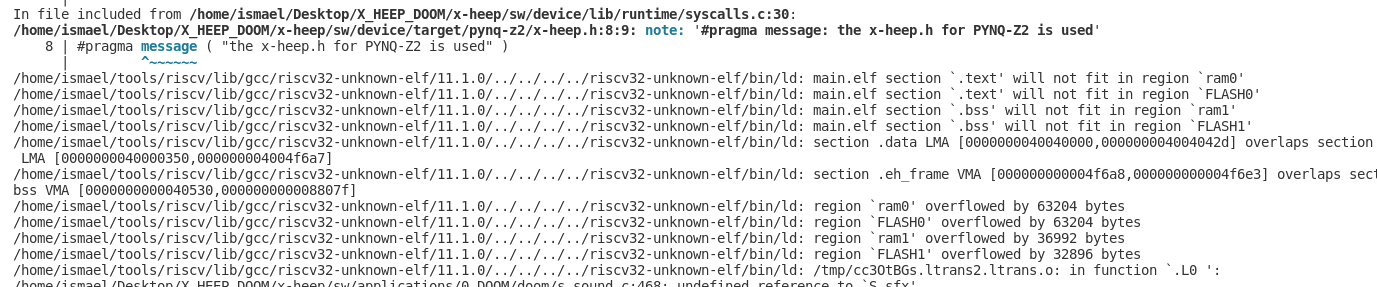
\includegraphics[width=\textwidth]{images/ramOverflowError.png}
    \caption{Error message of RAM overflow before it was optimized}
    \label{fig:ramOverflowError}
\end{figure}


\paragraph{Screen Buffers:} The first iteration of DOOM adapted for X-HEEP had three screen buffers. Two of them were the video buffer and back buffer from the original DOOM, each 320x200 pixels and paletted 8 bits per pixel. While the video buffer is written on the display, the back buffer is filled with the next frame. When both operations are finished, the two buffers switch role. The third buffer was for the ST7789 with a size of 200x200 pixels but 16 bits per pixel for an RGB565 color format. These three screen buffers alone used 203 kB of RAM. The first optimization was to delete the back buffer. In the current version of the X-HEEP implementation, the SPI transfer to the display is a blocking operation, meaning the CPU sends pixels one by one. Hence, there is no need for a back buffer, as no new image can be drawn into a buffer while another image is being drawn on the display. The second optimization was to delete the ST7789 screen buffer and convert paletted colors to RGB565 colors on the fly. As the CPU is already blocked anyway, it can also do the conversion before sending a pixel. This reduced the RAM usage of screen buffers by 141 kB, leaving 63 kB.


\paragraph{Augment RAM on FPGA:} The next step was to unblock all available memory banks on the FPGA. There are 16 memory banks with 32 kB each, totaling 512 kB of available memory. By default only two memory banks are activated for a total of 64kB. The available memory is divided into \texttt{ram0} for code and \texttt{ram1} for data. Activating all 16 memory banks on the FPGA gave acess to the whole 512kB of memory. The correct division between the two memories was found by adjusting settings in \texttt{configs/general.hjson} on lines 17 and 21. The final value that made it compile is \texttt{0x000053000}. This divides the available space into two parts of 332 kB for \texttt{ram0}, and 180 kB for \texttt{ram1}.


